\documentclass[]{standalone}
\usepackage{tikz}
\usetikzlibrary{shapes,arrows,calc,positioning}
\usepackage{amsmath} % for dfrac
\usepackage{comment}
\usepackage{calc}

% definition of basic block
\tikzset{
    block/.style = {draw, rectangle,
        minimum height=1.2cm,
        minimum width=2cm},
    input/.style = {coordinate,node distance=1cm},
    output/.style = {coordinate,node distance=1cm},
    sum/.style = {draw, circle, node distance=1cm},
}

% definition of saturation block
\tikzset{% from https://tex.stackexchange.com/questions/161075/saturation-block
  saturation block/.style={%
    draw, 
    path picture={
      % Get the width and height of the path picture node
      \pgfpointdiff{\pgfpointanchor{path picture bounding box}{north east}}%
        {\pgfpointanchor{path picture bounding box}{south west}}
      \pgfgetlastxy\x\y
      % Scale the x and y vectors so that the range
      % -1 to 1 is slightly shorter than the size of the node
      \tikzset{x=\x*.4, y=\y*.4}
      %
      % Draw annotation
      \draw (-1,0) -- (1,0) (0,-1) -- (0,1); 
      \draw (-1,-.7) -- (-.6,-.7) -- (.6,.7) -- (1,.7);
    }
  }
}
\tikzset{% from https://tex.stackexchange.com/questions/161075/saturation-block
  deadband block/.style={%
    draw, 
    path picture={
      % Get the width and height of the path picture node
      \pgfpointdiff{\pgfpointanchor{path picture bounding box}{north east}}%
        {\pgfpointanchor{path picture bounding box}{south west}}
      \pgfgetlastxy\x\y
      % Scale the x and y vectors so that the range
      % -1 to 1 is slightly shorter than the size of the node
      \tikzset{x=\x*.4, y=\y*.4}
      %
      % Draw annotation
      \draw (-1,0) -- (1,0) (0,-1) -- (0,1);  % axis
      \draw (-1,1) -- (-.3,.3) -- (-.3,0) -- (.3,0) -- (.3,-.3) -- (1,-1);
	  %\draw (-.3,.3) -- (.3,-.3) ;
    }
  }
}

\begin{document}
	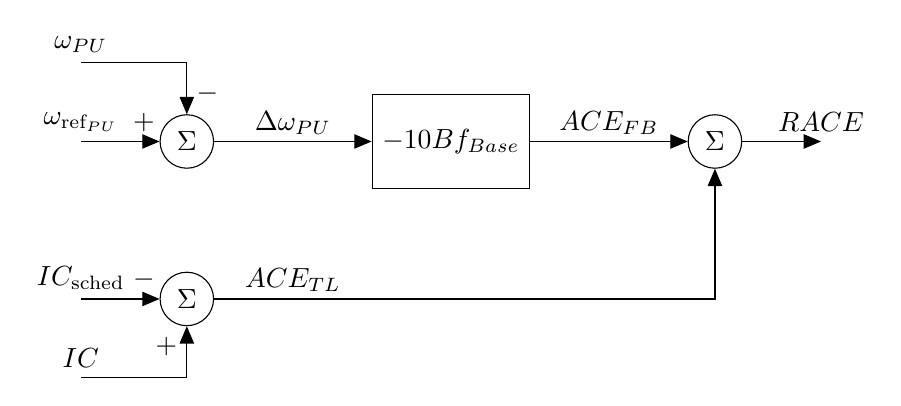
\begin{tikzpicture}[auto, node distance=1cm,>=triangle 45]
		% Starting inputwref
		\node [input, name=inputwref, label=$\omega_{\text{ref}_{PU}}$]  {};
		% Starting inputw
		\node [input, name=inputw, above=of inputwref, label=$\omega_{PU}$] (inputw) {};
		% sum 1
		\node [sum, right=of inputwref] (sum1) {$\Sigma$};
		% delta w node and label
		\coordinate [right=of sum1]  (deltaw) {};
		\coordinate [above=-.1em of deltaw,label={$\Delta\omega_{PU}$}]  (deltaWlabel){};
		
		% input ICsched
		\node [input, name=ICsched, below=2 cm of inputwref, label=$IC_{\text{sched}}$] {};
		% input IC
		\node [input, name=IC, below=of ICsched, label=$IC$] {};
		% sum 2
		\node [sum, right=of ICsched] (sum2) {$\Sigma$};
		% Tie Line ACE node and label
		\coordinate [right=of sum2]  (ACEtl) {};
		\coordinate [above=-.1em of ACEtl,label={$ACE_{TL}$}]  (ACEtllabel){};
		
		% Frequnecy Bias block
		\node [block, right=of deltaw] (fbias) {$-10Bf_{Base}$};
		% frequency Bias ACE node and label
		\coordinate [right=of fbias]  (ACEfb) {};
		\coordinate [above=-.1em of ACEfb,label={$ACE_{FB}$}]  (ACEfblabel){};
		
		% reported Summing
		\node [sum, right=of ACEfb,] (sum3) {$\Sigma$};

		% reported ACE out
		\node [output, right=of sum3, label=$RACE$] (output) {};
		
		% connecting lines
		\draw [draw,->] (inputwref) -- node[pos=0.8] {$+$} (sum1); 
		\draw [->] (inputw) -| node[pos=0.8] {$-$} (sum1);
		\draw [->] (sum1) -- (fbias);
		\draw [draw,->] (ICsched) -- node[pos=0.8] {$-$} (sum2); 
		\draw [->] (IC) -| node[pos=0.8] {$+$} (sum2);
		\draw [->] (fbias) -- (sum3);
		\draw [->] (sum2) -| (sum3.south); % using calc to find point halfway between corner and middle	
		\draw [->] (sum3) -- (output);
	
	\end{tikzpicture} 
\end{document}